\documentclass[14pt]{extbook}
\usepackage{multicol, enumerate, enumitem, hyperref, color, soul, setspace, parskip, fancyhdr} %General Packages
\usepackage{amssymb, amsthm, amsmath, latexsym, units, mathtools} %Math Packages
\everymath{\displaystyle} %All math in Display Style
% Packages with additional options
\usepackage[headsep=0.5cm,headheight=12pt, left=1 in,right= 1 in,top= 1 in,bottom= 1 in]{geometry}
\usepackage[usenames,dvipsnames]{xcolor}
\usepackage{dashrule}  % Package to use the command below to create lines between items
\newcommand{\litem}[1]{\item#1\hspace*{-1cm}\rule{\textwidth}{0.4pt}}
\pagestyle{fancy}
\lhead{Progress Quiz 5}
\chead{}
\rhead{Version B}
\lfoot{8497-6012}
\cfoot{}
\rfoot{Summer C 2021}
\begin{document}

\begin{enumerate}
\litem{
Solve the radical equation below. Then, choose the interval(s) that the solution(s) belongs to.\[ \sqrt{3 x - 8} - \sqrt{8 x - 9} = 0 \]\begin{enumerate}[label=\Alph*.]
\item \( \text{All solutions lead to invalid or complex values in the equation.} \)
\item \( x \in [-5.7,-1.7] \)
\item \( x_1 \in [-2, 1] \text{ and } x_2 \in [0.67,4.67] \)
\item \( x_1 \in [0.3, 3.6] \text{ and } x_2 \in [0.67,4.67] \)
\item \( x \in [-2,1] \)

\end{enumerate} }
\litem{
Choose the graph of the equation below.\[ f(x) = \sqrt[3]{x + 6} + 6 \]\begin{enumerate}[label=\Alph*.]
\begin{multicols}{2}\item 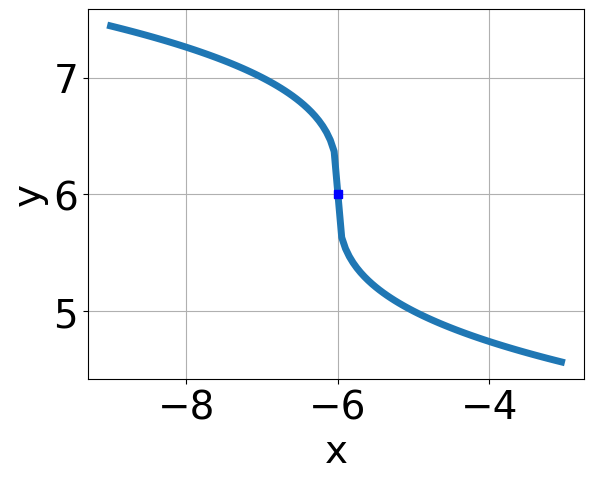
\includegraphics[width = 0.3\textwidth]{../Figures/radicalEquationToGraphCopyAB.png}\item 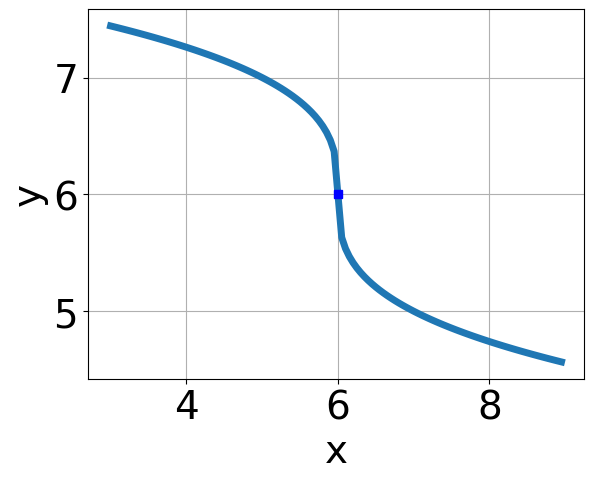
\includegraphics[width = 0.3\textwidth]{../Figures/radicalEquationToGraphCopyBB.png}\item 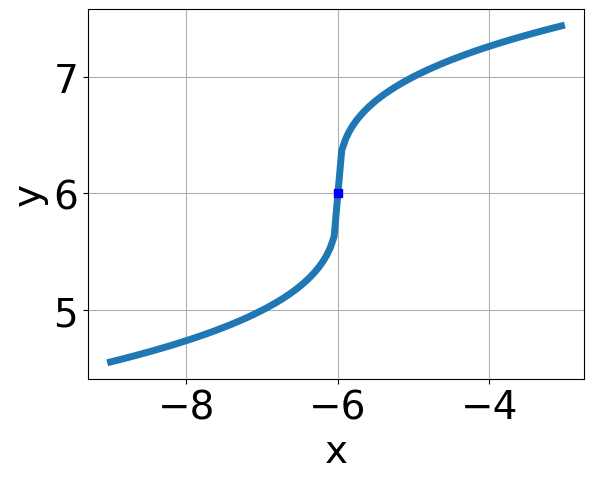
\includegraphics[width = 0.3\textwidth]{../Figures/radicalEquationToGraphCopyCB.png}\item 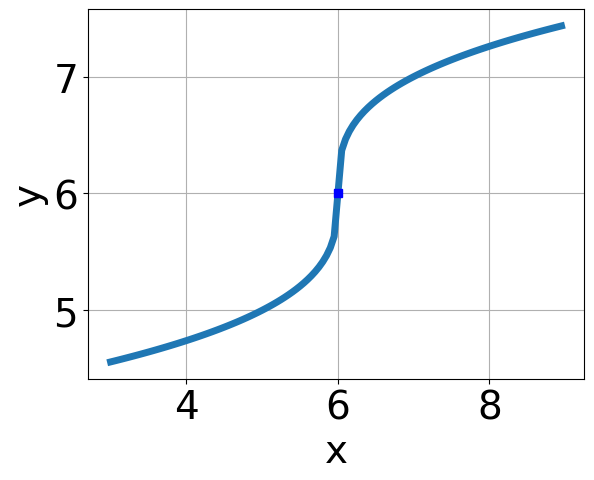
\includegraphics[width = 0.3\textwidth]{../Figures/radicalEquationToGraphCopyDB.png}\end{multicols}\item None of the above.
\end{enumerate} }
\litem{
Choose the equation of the function graphed below.
\begin{center}
    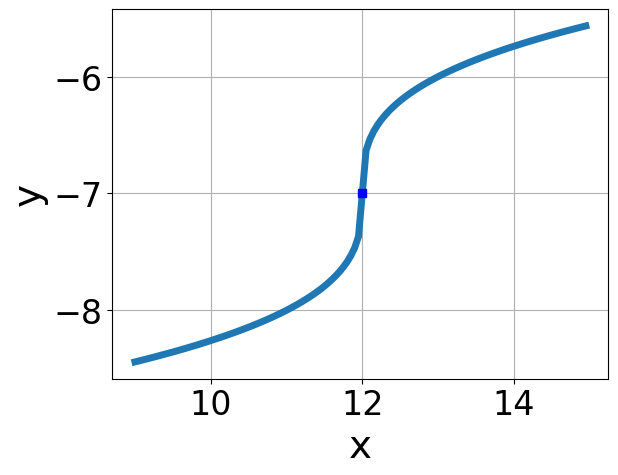
\includegraphics[width=0.5\textwidth]{../Figures/radicalGraphToEquationB.png}
\end{center}
\begin{enumerate}[label=\Alph*.]
\item \( f(x) = \sqrt[3]{x + 12} - 7 \)
\item \( f(x) = \sqrt[3]{x - 12} - 7 \)
\item \( f(x) = - \sqrt[3]{x + 12} - 7 \)
\item \( f(x) = - \sqrt[3]{x - 12} - 7 \)
\item \( \text{None of the above} \)

\end{enumerate} }
\litem{
Solve the radical equation below. Then, choose the interval(s) that the solution(s) belongs to.\[ \sqrt{21 x^2 + 32} - \sqrt{-52 x} = 0 \]\begin{enumerate}[label=\Alph*.]
\item \( x_1 \in [0.9, 1.23] \text{ and } x_2 \in [0,1.9] \)
\item \( x \in [-1.34,-1.22] \)
\item \( \text{All solutions lead to invalid or complex values in the equation.} \)
\item \( x_1 \in [-1.34, -1.22] \text{ and } x_2 \in [-2.7,-0.4] \)
\item \( x \in [-1.3,-0.99] \)

\end{enumerate} }
\litem{
Solve the radical equation below. Then, choose the interval(s) that the solution(s) belongs to.\[ \sqrt{-4 x - 7} - \sqrt{7 x - 4} = 0 \]\begin{enumerate}[label=\Alph*.]
\item \( x \in [-0.88,-0.19] \)
\item \( x_1 \in [-2.12, -1.61] \text{ and } x_2 \in [0.4,2] \)
\item \( x_1 \in [-2.12, -1.61] \text{ and } x_2 \in [-1.8,0] \)
\item \( \text{All solutions lead to invalid or complex values in the equation.} \)
\item \( x \in [-1.08,-0.42] \)

\end{enumerate} }
\litem{
What is the domain of the function below?\[ f(x) = \sqrt[6]{7 x - 9} \]\begin{enumerate}[label=\Alph*.]
\item \( [a, \infty), \text{ where } a \in [1.19, 1.4] \)
\item \( (-\infty, \infty) \)
\item \( [a, \infty), \text{where } a \in [0.44, 1.13] \)
\item \( (-\infty, a], \text{where } a \in [1.02, 1.96] \)
\item \( (-\infty, a], \text{where } a \in [0.33, 1] \)

\end{enumerate} }
\litem{
Choose the graph of the equation below.\[ f(x) = - \sqrt[3]{x - 6} + 7 \]\begin{enumerate}[label=\Alph*.]
\begin{multicols}{2}\item 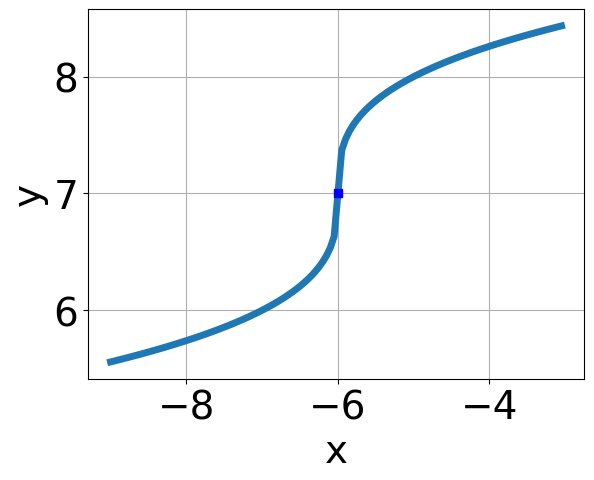
\includegraphics[width = 0.3\textwidth]{../Figures/radicalEquationToGraphAB.png}\item 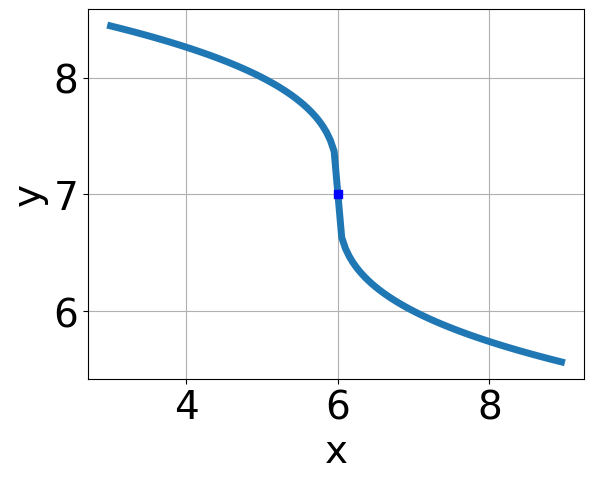
\includegraphics[width = 0.3\textwidth]{../Figures/radicalEquationToGraphBB.png}\item 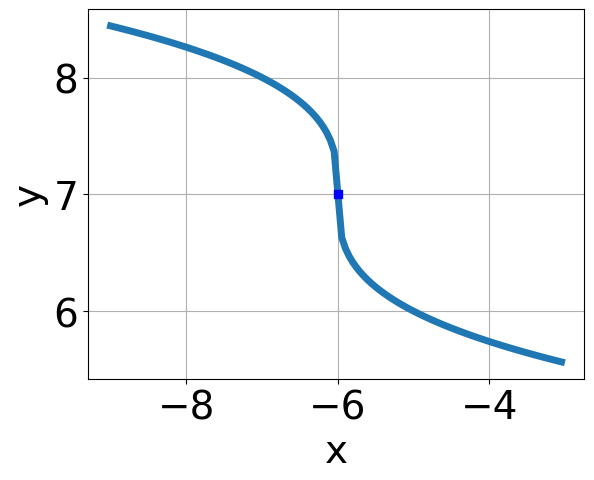
\includegraphics[width = 0.3\textwidth]{../Figures/radicalEquationToGraphCB.png}\item 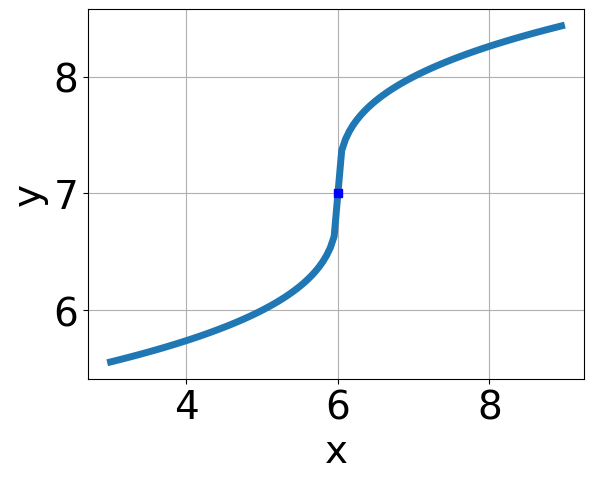
\includegraphics[width = 0.3\textwidth]{../Figures/radicalEquationToGraphDB.png}\end{multicols}\item None of the above.
\end{enumerate} }
\litem{
Choose the equation of the function graphed below.
\begin{center}
    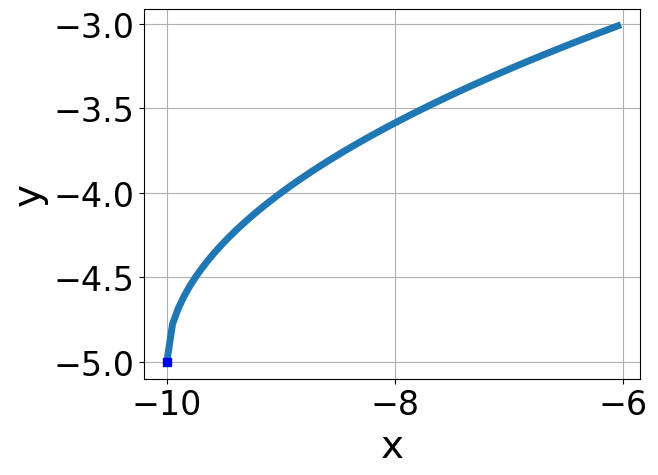
\includegraphics[width=0.5\textwidth]{../Figures/radicalGraphToEquationCopyB.png}
\end{center}
\begin{enumerate}[label=\Alph*.]
\item \( f(x) = - \sqrt[3]{x + 10} - 5 \)
\item \( f(x) = \sqrt[3]{x - 10} - 5 \)
\item \( f(x) = - \sqrt[3]{x - 10} - 5 \)
\item \( f(x) = \sqrt[3]{x + 10} - 5 \)
\item \( \text{None of the above} \)

\end{enumerate} }
\litem{
Solve the radical equation below. Then, choose the interval(s) that the solution(s) belongs to.\[ \sqrt{21 x^2 - 20} - \sqrt{13 x} = 0 \]\begin{enumerate}[label=\Alph*.]
\item \( x \in [1.14,1.36] \)
\item \( x \in [-1.67,-0.1] \)
\item \( x_1 \in [-1.67, -0.1] \text{ and } x_2 \in [-3.67,4.33] \)
\item \( \text{All solutions lead to invalid or complex values in the equation.} \)
\item \( x_1 \in [0.36, 1.29] \text{ and } x_2 \in [-3.67,4.33] \)

\end{enumerate} }
\litem{
What is the domain of the function below?\[ f(x) = \sqrt[6]{8 x - 4} \]\begin{enumerate}[label=\Alph*.]
\item \( [a, \infty), \text{where } a \in [1.32, 2.07] \)
\item \( (-\infty, \infty) \)
\item \( (-\infty, a], \text{where } a \in [1.5, 3.9] \)
\item \( [a, \infty), \text{ where } a \in [-0.56, 0.57] \)
\item \( (-\infty, a], \text{where } a \in [-0.1, 0.6] \)

\end{enumerate} }
\end{enumerate}

\end{document}